\documentclass[main.tex]{subfiles}
 
\begin{document}

\part{Slow slip}

\chapter{Introduction}

\begin{itemize}
	\item Some generalities about slow slip and tremor
	\item A few words about what wavelets are
	\item Short bibliography about what has been done (master Seqoia Alba + papers by Ohtani and Wei)
\end{itemize}

The goal of this research work is to study the changes over time in the spectral content of recordings of surface displacement by GPS stations, in order to detect slow slip events. We hope that by combining wavelet analyses of several channels and several stations, we will be able to detect smaller inter-ETS events, which can currently be observed in the tremor catalogs, but not in the GPS data.

\chapter{Data}

We use the GPS data collected and made available on the website of the Pacific Northwest Geodetic Array (\href{http://www.geodesy.cwu.edu/}{PANGA}), from Central Washington University. Three types of time series are available:

\begin{itemize}
\item Raw data recorded by the GPS stations, after GIPSY postprocessing.
\item Detrended data, for which a linear trend corresponding to the secular plate motion has been removed from the data.
\item Cleaned data, for which the linear trend, steps due to earthquakes or hardware upgrades, and annual and semi-annual sinusoids signals have been simultaneously estimated and removed following Szeliga \textit{et al.} (2008 ~\cite{SZE_2008}). Surface loading due to hydrology and atmospheric pressure introduces an annual signal in the GPS time series with respect to a global reference frame. This annually repeating component also introduces power at all harmonic frequencies, thus it may also be necessary to remove a semi-annual sinusoid from the raw data (Blewitt and Lavall\'ee, 2002 ~\cite{BLE_2002}).
\end{itemize}

For each GPS station, the website provides a file for the three components of the displacement (latitude, longitude, and vertical), and each file contains three columns, corresponding to the time, the displacement (in millimetres), and the error. The data are recorded once a day. \\

The raw data are filtered with the function $f (t)$ to obtain the detrended, and then the cleaned data:

\begin{equation}
f (t) = \textrm{line} (t) + \textrm{annual + semi-annual} (t) + \textrm{jumps} (t)
\end{equation}

with:

\begin{equation}
\textrm{line} (t) = p_1 + p_2 t
\end{equation}

\begin{equation}
\textrm{annual + semi-annual} (t) = p_3 \sin (2 \pi t + p_4) + p_5 \sin (4 \pi t + p_6)
\end{equation}

\begin{equation}
\textrm{jumps} (t) = \sum_{i = 1}^{n} p_i \textrm{Heaviside} (t - t_i)
\end{equation}

The values of the $p_i$ and $t_i$ are given at the beginning of each file. The best linear unbiased estimate of the model parameters $p_i$ are computed using an orthogonal-triangular decomposition, or QR-factorization (Nikolaidis, 2002 ~\cite{NIK_2002}).

\chapter{Method}

The Discrete Wavelet Transform (DWT) is an orthonormal transform that uses a sequence of filtering operations to associate a time series $X_t (t = 0 , ... , N - 1)$ written in the traditional orthonormal basis:

\begin{equation}
\bm{X} = X_0 \begin{pmatrix} 1 \\ 0 \\ 0 \\ . \\ . \\ . \\ 0 \end{pmatrix}
+ X_1 \begin{pmatrix} 0 \\ 1 \\ 0 \\ . \\ . \\ . \\ 0 \end{pmatrix}
+ X_2 \begin{pmatrix} 0 \\ 0 \\ 1 \\ . \\ . \\ . \\ 0 \end{pmatrix}
+ ... + X_{N - 1} \begin{pmatrix} 0 \\ 0 \\ 0 \\ . \\ . \\ . \\ 1 \end{pmatrix}
\end{equation}

with the wavelet coefficients $W_t (t = 0 , ... , N - 1)$, which is the same time series written in another orthonormal basis:

\begin{equation}
\bm{X} = W_0 \begin{pmatrix} \mathcal{W}_{0 , 0} \\ \mathcal{W}_{0 , 1} \\ \mathcal{W}_{0 , 2} \\ . \\ . \\ . \\ \mathcal{W}_{0 , N - 1} \end{pmatrix}
+ W_1 \begin{pmatrix} \mathcal{W}_{1 , 0} \\ \mathcal{W}_{1 , 1} \\ \mathcal{W}_{1 , 2} \\ . \\ . \\ . \\ \mathcal{W}_{1 , N - 1} \end{pmatrix}
+ W_2 \begin{pmatrix} \mathcal{W}_{2 , 0} \\ \mathcal{W}_{2 , 1} \\ \mathcal{W}_{2 , 2} \\ . \\ . \\ . \\ \mathcal{W}_{2 , N - 1} \end{pmatrix}
+ ... + W_{N - 1} \begin{pmatrix} \mathcal{W}_{N - 1 , 0} \\ \mathcal{W}_{N - 1 , 1} \\ \mathcal{W}_{N - 1 , 2} \\ . \\ . \\ . \\ \mathcal{W}_{N - 1 , N - 1} \end{pmatrix}
\end{equation}

where the $\bm{\mathcal{W}_{t , .}} \left( t = 0 , ... , N - 1 \right)$ are the wavelet basis vectors. The main advantage of the wavelet transform is that it captures information about both the frequency and the temporal content of the input data. This is contrasted with the Fourier transform, which characterizes the amplitude and phase of the frequency content only. Indeed, a local perturbation of the initial time series will affect all the coefficients of the Fourier transform, whereas it will only affect a few wavelet coefficients around the time of the perturbation. \\ 

The first $\frac{N}{2}$ $\bm{\mathcal{W}_{t , .}} \left( t = 0 , ... , \frac{N}{2} - 1 \right)$ wavelet basis vectors are circularly shifted with each other:

\begin{equation}
\mathcal{W}_{k , j} = \mathcal{W}_{i , j + 2 \left( i - k \right)}
\end{equation}

and their Fourier transform has a nominal frequency band of $\lbrack \frac{1}{4 dt} ; \frac{1}{2 dt} \rbrack$, where $dt$ is the time step of the time series. We can write their coordinates as:

\begin{equation}
\mathcal{W}_{t , l} = h_{2 t + 1 - l \mod N} \text{, } t = 0 , ... , \frac{N}{2} - 1 \text{, } l = 0 , ... , N - 1
\end{equation}

where $h_l \left( l = 0 , ... , N - 1 \right)$ is the wavelet filter. \\

The first wavelet vector $\bm{W_1}$ has length $\frac{N}{2}$, and is associated with changes on scale $\tau_1 = dt$. We can get its coefficients $W_{1 , t} \left(t = 0 , ... , \frac{N}{2} - 1 \right)$ by computing the scalar product of the first $\frac{N}{2}$ $\bm{\mathcal{W}_{t , .}} \left( t = 0 , ... , \frac{N}{2} - 1 \right)$ wavelet basis vectors with the time series $\bm{X}$:

\begin{equation}
W_{1 , t} = \sum_{j = 0}^{N - 1} \mathcal{W}_{t , j} X_j \text{, } t = 0 , ... , \frac{N}{2} - 1
\end{equation}

The new time series $\bm{W_1}$ has time step $2 dt$, and corresponds to the filtering of the original time series with a filter with nominal frequency interval $\lbrack \frac{1}{4 dt} ; \frac{1}{2 dt} \rbrack$. \\

The next $\frac{N}{4}$ $\bm{\mathcal{W}_{t , .}} \left( t = \frac{N}{2} , .... , \frac{3 N}{4} - 1 \right)$ wavelet basis vectors are also circularly shifted with each other:

\begin{equation}
\mathcal{W}_{k , j} = \mathcal{W}_{i , j + 4 \left( i - k \right)}
\end{equation}

and their Fourier transform has a nominal frequency band of $\lbrack \frac{1}{8 dt} ; \frac{1}{4 dt} \rbrack$. We can write their coordinates as:

\begin{equation}
\mathcal{W}_{\frac{N}{2} + t , l} = \sum_{j = 0}^{N - 1} g_{j - l \mod N} h_{4 t + 3 - j \mod N}^{\uparrow} \text{, } t = 0 , ... , \frac{N}{4} - 1 \text{, } l = 0 , ... , N - 1
\end{equation}

where $\bm{h^{\uparrow}}$ is formed by inserting a $0$ between each of the elements of $\bm{h}$, and $g_l \left( l = 0 , ... , N - 1 \right)$ is the scaling filter defined by:

\begin{equation}
g_l = \left( - 1 \right) ^{l + 1} h_{N - 1 - l} \text{, } l = 0 , ... , N - 1
\end{equation}

The second wavelet vector $\bm{W_2}$ has length $\frac{N}{4}$, and is associated with changes on scale $\tau_2 = 2 dt$. We can get its coefficients $W_{2 , t} \left( t = 0 , ... , \frac{N}{4} - 1 \right)$ by computing the scalar product of the next $\frac{N}{4}$ $\bm{\mathcal{W}_{t , .}} \left( t = \frac{N}{2} , ... , \frac{3 N}{4} - 1 \right)$ wavelet basis vectors with the time series $\bm{X}$:

\begin{equation}
W_{2 , t} = \sum_{j = 0}^{N - 1} \mathcal{W}_{\frac{N}{2} + t , j} X_j \text{, } t = 0 , ... , \frac{N}{4} - 1
\end{equation}

The new time series $\bm{W_2}$ has time step $4 dt$, and corresponds to the filtering of the original time series with a filter with nominal frequency interval $\lbrack \frac{1}{8 dt} ; \frac{1}{4 dt} \rbrack$. \\

At the level $J$, we can write the orthonormal transform as:

\begin{equation}
\bm{W} = \mathcal{W} \bm{X} \text{ or } \begin{pmatrix} \bm{W_1} \\ \bm{W_2} \\ \bm{W_3} \\ . \\ . \\ . \\ \bm{W_J} \\ \bm{V_J} \end{pmatrix}
= \begin{pmatrix} \mathcal{W}_1 \bm{X} \\ \mathcal{W}_2 \bm{X} \\ \mathcal{W}_3 \bm{X} \\ . \\ . \\ . \\ \mathcal{W}_J \bm{X} \\ \mathcal{V}_J \bm{X} \end{pmatrix}
\end{equation}

Each of the wavelet vectors $\bm{W_j} \left( j = 1 , ... , J \right)$ has length $\frac{N}{2^j}$, has a time step of $2^j dt$, and corresponds to the filtering of the initial time series by a filter of nominal frequency band $\lbrack \frac{1}{dt 2^{j + 1}} ; \frac{1}{dt 2^j} \rbrack$. The scaling vector $\bm{V_J}$ has length $\frac{N}{2^J}$, has a time step of $2^J dt$, and corresponds to the filtering of the initial time series by a filter of nominal frequency band $\lbrack 0 ; \frac{1}{dt 2^{J + 1}} \rbrack$. \\

We can compute iteratively the wavelet vectors and the scaling vector using a pyramid algorithm and the wavelet filter $h_l \left( l = 0 , ... , N - 1 \right)$ and the scaling filter $g_l \left( l = 0 , ... , N - 1 \right)$:

\begin{equation}
W_{j , t} = \sum_{l = 0}^{N - 1} h_l V_{j - 1 , 2 t + 1 - l \mod N_{j - 1}} \text{ and } V_{j , t} = \sum_{l = 0}^{N - 1} g_l V_{j - 1 , 2 t + 1 - l \mod N_{j - 1}} \text{, } t = 0 , ... , N_j - 1
\end{equation}

where $N_j = \frac{N}{2^j}$ and $\bm{V_0} = \bm{X}$. \\

We can then compute the $j$th level detail $\bm{D_j} \left( j = 1 , ... , J \right)$, which is a vector of length $N$, defined by $\bm{D_j} = \mathcal{W}_j^T \bm{W_j}$ and the $J$th level smooth $\bm{S_J}$, which is a vector of length $N$, defined by $\bm{S_J} = \mathcal{V}_J^T \bm{V_J}$, and we get the multiresolution analysis (MRA) of $\bm{X}$:

\begin{equation}
\bm{X} = \sum_{j = 1}^{J} \bm{D_j} + \bm{S_J}
\end{equation}

One main advantage of the DWT is that it is an orthonormal transform, and thus we can write the analysis of variance (ANOVA):

\begin{equation}
\left\Vert \bm{X} \right\Vert ^2 = \left\Vert \bm{W} \right\Vert ^2 = \sum_{j = 1}^{J} \left\Vert \bm{W_j} \right\Vert ^2 + \left\Vert \bm{V_J} \right\Vert ^2 = \sum_{j = 1}^{J} \left\Vert \bm{D_j} \right\Vert ^2 + \left\Vert \bm{S_J} \right\Vert ^2
\end{equation}

Moreover, the DWT can be computed using $O \left( N \right)$ multiplications. \\

However, the DWT present several disadvantages:

\begin{itemize}
	\item The length of the time series must be a multiple of $2^J$ where $J$ is the level of the DWT decomposition.
	\item The time step of the wavelet vector $\bm{W_j}$ is $2^j dt$, which may not correspond to the time when some interesting phenomenon is visible on the original time series.
	\item When we circularly shift the time series, the corresponding wavelet coefficients, details and smooths are not a circularly shifted version of the wavelet coefficients, details and smooths of the original time series. Thus, the values of the wavelet coefficients, details and smooths are strongly dependent on the time when we start experimentally gathering the data.
	\item When we filter the time series to obtain the details and smooths, we introduce a phase shift, which makes difficult to line up meaningfully the features of the MRA with the original time series.
\end{itemize}

To get rid of these problems, we introduce the Maximum Overlap Discrete Wavelet Transform (MODWT). The MODWT transforms the time series $X_t \left( t = 0, ... , N - 1 \right)$ into J wavelet vectors $\bm{\widetilde{W}_j} \left( j = 1 , ... , J \right)$ of length $N$ and a scaling vector $\bm{\widetilde{V}_J}$ of length $N$. Each wavelet vector $\bm{\widetilde{W}_j}$ corresponds to the filtering of the original time series with a filter with nominal frequency band $\lbrack \frac{1}{dt 2^{j + 1}} ; \frac{1}{dt 2^j} \rbrack$. The scaling vector $\bm{\widetilde{V}_J}$ corresponds to the filtering of the original time series with a filter with nominal frequency interval $\lbrack 0 ; \frac{1}{dt 2^{j + 1}} \rbrack$.

We can write the transformation as:

\begin{equation}
\bm{\widetilde{W}_j} = \widetilde{\mathcal{W}_j} \bm{X} \text{ and } \bm{\widetilde{V}_J} = \widetilde{\mathcal{V}_J} \bm{X}
\end{equation}

$ \widetilde{\mathcal{W}_j}$ and $\widetilde{\mathcal{V}_J}$ are related to $\mathcal{W}_j$ and $\mathcal{V}_J$ by:

\begin{equation}
\widetilde{\mathcal{W}}_{j, t l} = \widetilde{h}_{j , t - l \mod N} \text{, } \mathcal{W}_{j, t l} = h_{j , 2^j \left( t + 1 \right) - 1 - l \mod N} \text{ and } \widetilde{h}_{j , l} = \frac{h_{j , l}}{2^{j/2}}
\end{equation}

As is the case for the DWT, we can compute iteratively the MODWT wavelet vectors and the scaling vector using a pyramid algorithm and the wavelet filter $\widetilde{h}_l \left( l = 0 , ... , N - 1 \right)$ and the scaling filter $\widetilde{g}_l \left( l = 0 , ... , N - 1 \right)$:

\begin{equation}
\widetilde{W}_{j , t} = \sum_{l = 0}^{N - 1} \widetilde{h}_l V_{j - 1 , t - 2^{j - 1} l \mod N} \text{ and } \widetilde{V}_{j , t} = \sum_{l = 0}^{N - 1} \widetilde{g}_l V_{j - 1 , t - 2^{j - 1} l \mod N} \text{, } t = 0 , ... , N - 1
\end{equation}

where $\widetilde{h}_l = \frac{h_l}{\sqrt{2}} \left( l = 0 , ... , N - 1 \right)$,  $\widetilde{g}_l = \frac{g_l}{\sqrt{2}} \left( l = 0 , ... , N - 1 \right)$ and $\bm{\widetilde{V}_0} = \bm{X}$. \\

We can then compute the $j$th level detail $\bm{\widetilde{D_j}} \left( j = 1 , ... , J \right)$, which is a vector of length $N$, defined by $\bm{\widetilde{D_j}} = \widetilde{\mathcal{W}_j}^T \bm{\widetilde{W_j}}$ and the $J$th level smooth $\bm{\widetilde{S_J}}$, which is a vector of length $N$, defined by $\bm{\widetilde{S_J}} = \widetilde{\mathcal{V}_J}^T \bm{\widetilde{V_J}}$, and we get the multiresolution analysis (MRA) of $\bm{X}$:

\begin{equation}
\bm{X} = \sum_{j = 1}^{J} \bm{\widetilde{D_j}} + \bm{\widetilde{S_J}}
\end{equation}

and the ANOVA:

\begin{equation}
\left\Vert \bm{X} \right\Vert ^2 = \sum_{j = 1}^{J} \left\Vert \bm{\widetilde{W}_j} \right\Vert ^2 + \left\Vert \bm{\widetilde{V}_J} \right\Vert ^2
\end{equation}

Now, we have the following properties:

\begin{itemize}
	\item The MODWT of a time series can be defined for any length $N$.
	\item The time step of the wavelet vectors $\bm{\widetilde{W}_j}$ and the scaling vector $\bm{\widetilde{V}_J}$ is equal to the time step of the original time series.
	\item When we circularly shift the time series, the corresponding wavelet vectors, scaling vector, details and smooths are shifted by the same amount.
	\item The details and smooths are associated with a zero phase filter, making it easy to line up meaningfully the features of the MRA with the original time series.
\end{itemize}

However, the MODWT has some disadvantages over the DWT:

\begin{itemize}
	\item The MODWT can only be computed using $O \left( N \log_2 N \right)$ multiplications.
	\item We can no longer write the ANOVA for the details and smooths:

\begin{equation}
\left\Vert \bm{X} \right\Vert ^2 \neq \sum_{j = 1}^{J} \left\Vert \bm{\widetilde{D_j}} \right\Vert ^2 + \left\Vert \bm{\widetilde{S_J}} \right\Vert ^2 \text{ and } \left\Vert \bm{\widetilde{W}_j} \right\Vert ^2 \neq \left\Vert \bm{\widetilde{D}_j} \right\Vert ^2
\end{equation}

\end{itemize}

\chapter{Results}

In the following, we show results of the DWT and MODWT analysis of one GPS time series. \\

Computing the DWT or the MODWT of a time series requires computing the convolution product of the time series with the wavelet or the scaling filter. To handle the boundary conditions, we assume that the time series is periodic, and extend accordingly the time series. However, we can only make this assumption when the discontinuity between the beginning and the end of the time series remains small. Therefore, we used the cleaned dataset in order to avoid discontinuities due to the linear trend, and earthquakes or hardware upgrades. In order to analyze the temporal correlation of the slow slip with the tectonic tremor, we also used the tremor catalog of the PNSN (Wech, 2010 ~\cite{WEC_2010}) to get the cumulative number of tremor recorded around the GPS station. The displacement is recorded once a day at every GPS station. However, there are many missing data points. We chose the GPS station PGC5, located in southern Vancouver Island, near Victoria. The slow slip events are clearly visible in the longitudinal component of the displacement (see bottom panel of Figure 20.1). Moreover, there are very few missing data for this station. In the following, we have analyzed eight years of GPS data from 2006 to 2014. There are only five days for which the displacement is missing. We replaced the missing data by the average of the displacement on the day before and the displacement on the day after. \\

We first carried out a partial DWT of the time series. To choose the appropriate wavelet filter, we computed the Normalized Partial Energy Sequence (NPES) of the wavelet coefficients and of the time series for different wavelet filters. It did not seem that there was much difference between the different wavelet filters. In the following, we will compare the wavelet coefficients to the cumulative number of tremor recorded around the GPS station. Therefore, we would like to know with good precision the time shift that should be applied to the wavelet coefficients. Moreover, we would like the length of the wavelet filter to remain small, in order to reduce the number of coefficients that are affected by the interpolation we had to do to replace the missing data. This is why we chose the LA8 wavelet filter in the following analysis. \\

The total duration of a slow slip event is about six weeks. Therefore, we only carried out a partial DWT up to the level 6 (corresponding to a scale of 64 days), because we do not expect to see features at a longer scale in the time series. \\

The wavelet coefficients for level 1 to 6 are shown in Figure 20.1. The red bars correspond to the days where data were missing. The grey bars correspond to the timing of ETS events.  We can clearly see big wavelet coefficients corresponding to the January 2007 ETS event at the levels 5 and 6, to the May 2009 ETS event at the level 5, to the August 2010 ETS event at the level 6, to the September 2012 ETS event at the levels 5 and 6, and to the September 2013 ETS event at the levels 5 and 6.  The May 2008 and August 2011 ETS events are not clearly seen in the wavelet coefficients. \\

\begin{center}
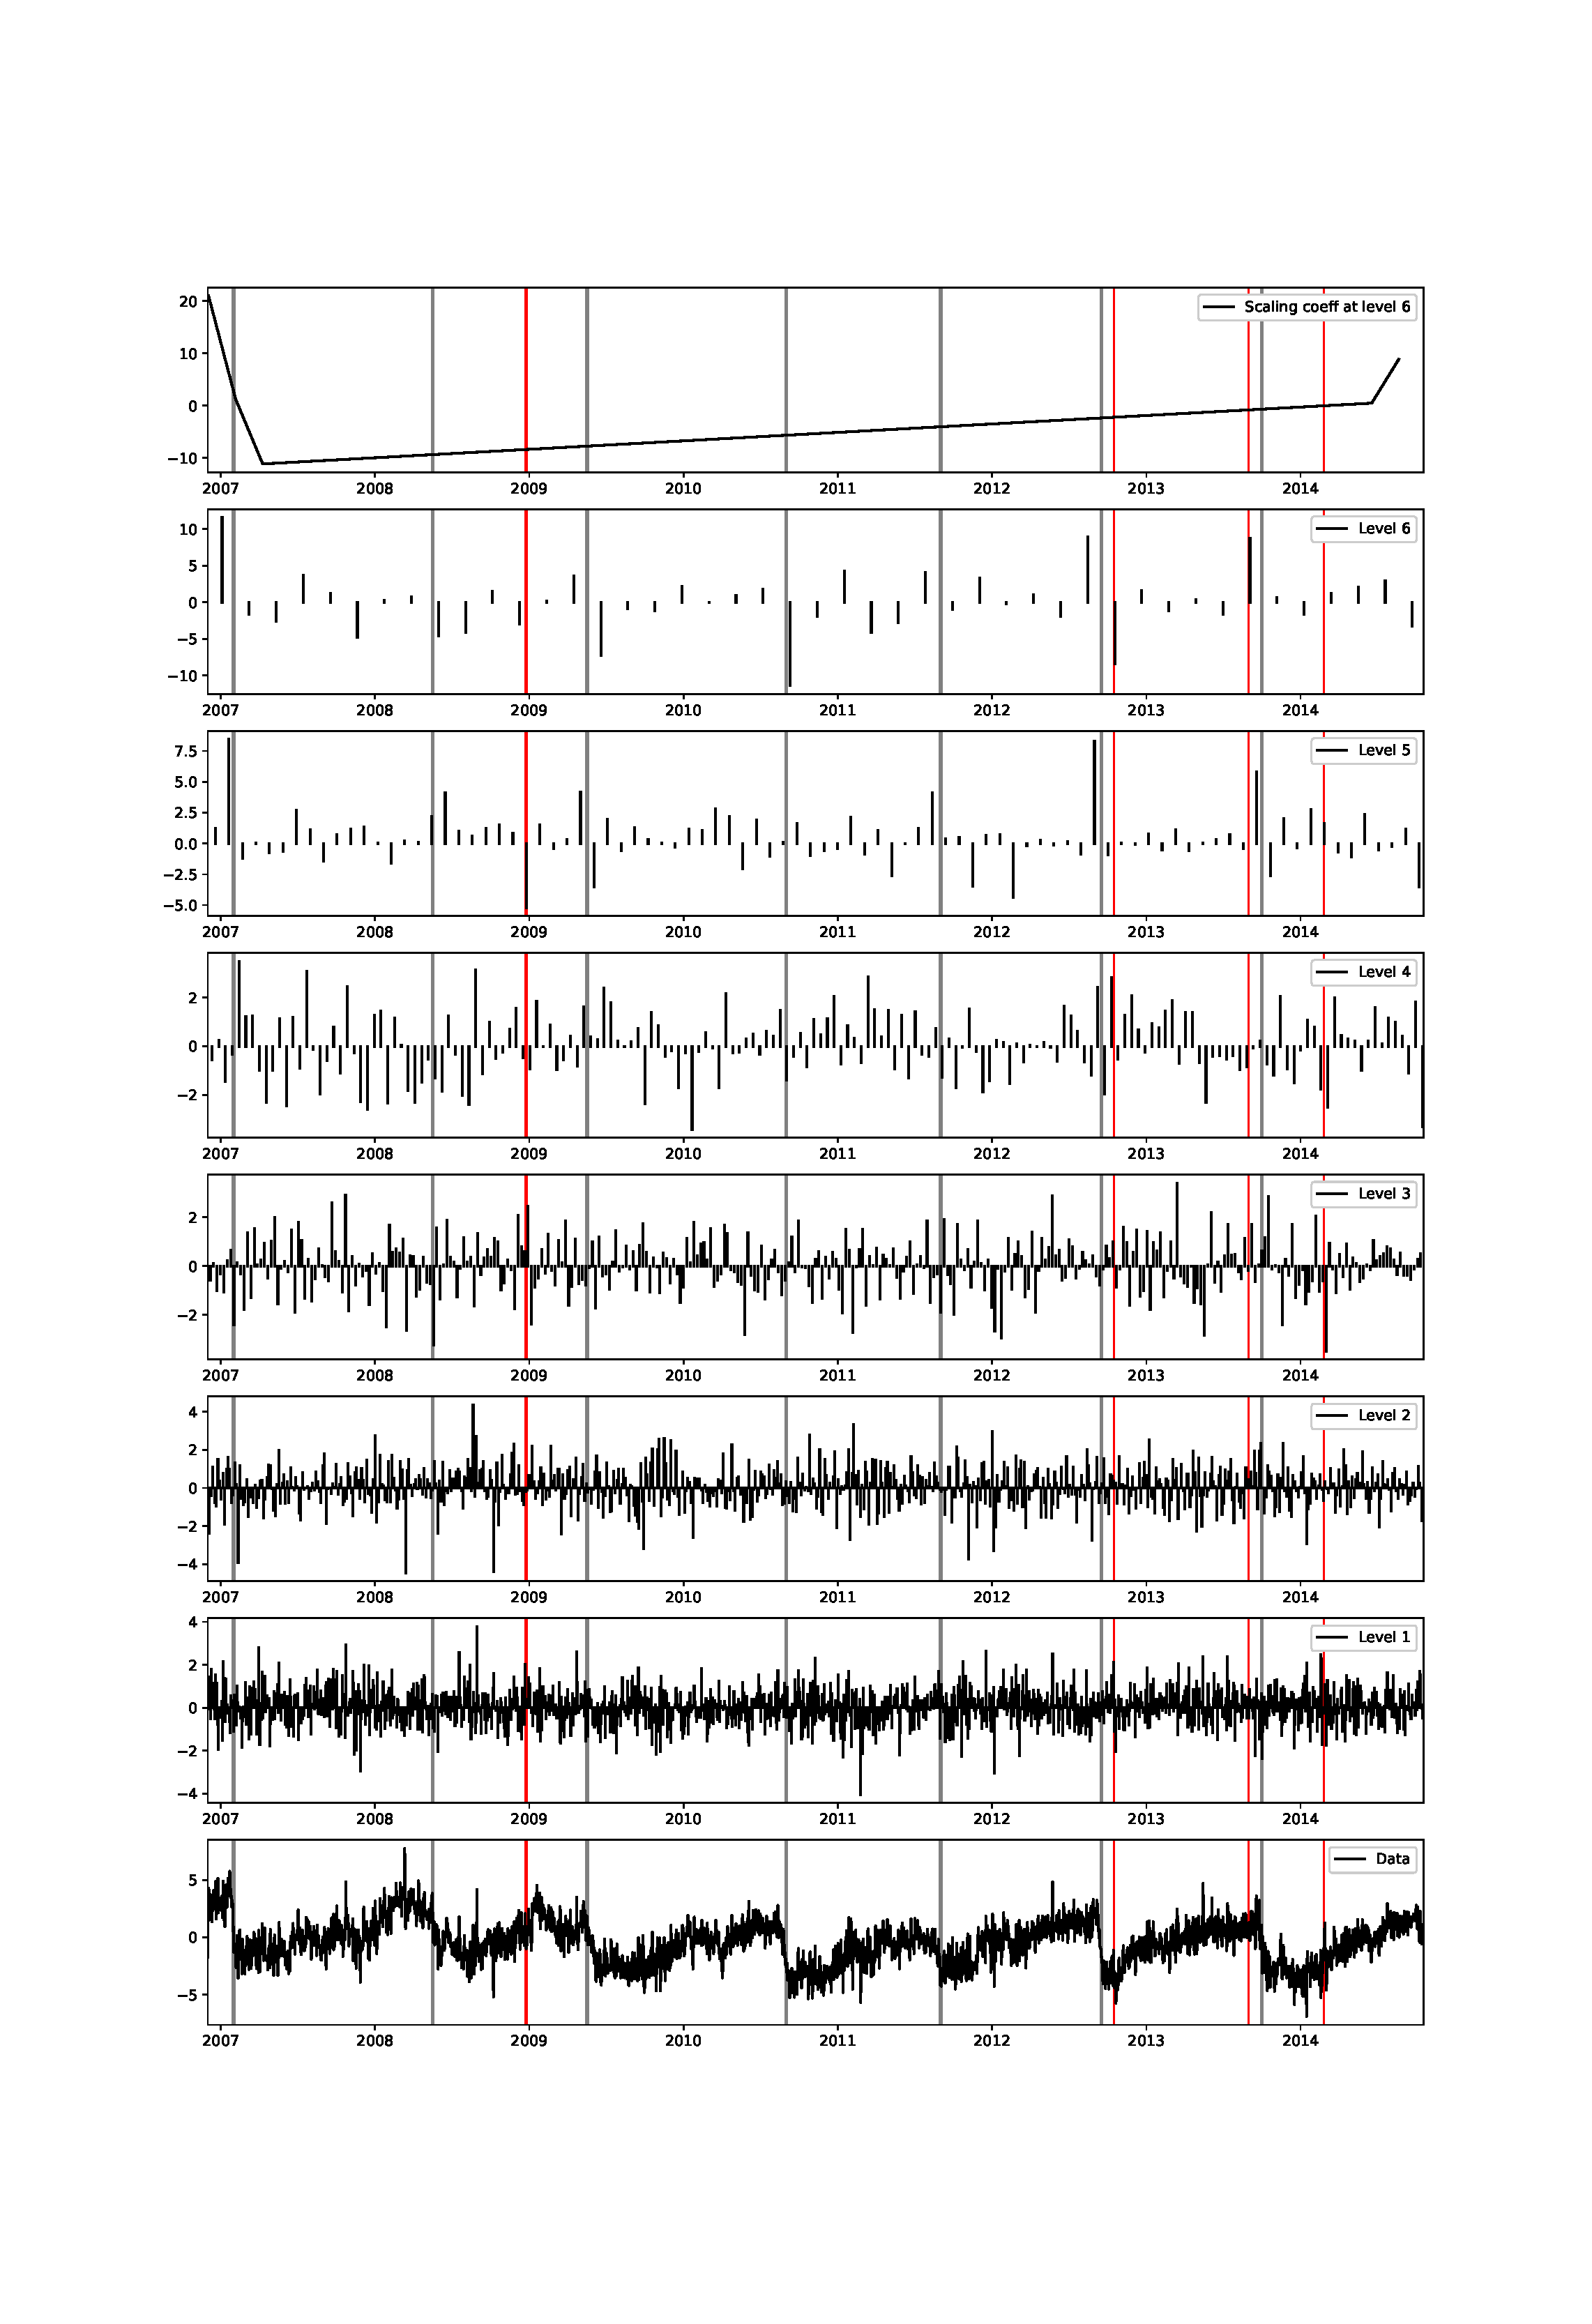
\includegraphics[width=300pt, trim={3.5cm 6cm 3.5cm 6.5cm},clip]{Figures/slowslip_results/Figure_1.eps}
\captionsetup{type=figure}
\captionof{figure}{Partial DWT wavelet coefficients up to level 6 of the longitudinal component of station PGC5. The red bars correspond to the days where data were missing. The grey bars correspond to the timing of ETS events.}
\end{center}

The 5\textsuperscript{th} and 6\textsuperscript{th} level details of the MRA are plotted with the cumulative number of tremor in Figure 20.2. Unfortunately, the tremor catalog from the PNSN website only starts in August 2009. As the GPS station is located at latitude N48\degree39', we only took into account the tremor which source was located between latitude N47.5\degree and latitude N49.5\degree. We can clearly see the August 2010, September 2012 and September 2013 ETS events in the 6\textsuperscript{th} level detail. The August 2010 ETS event is less obvious, but can be seen in the 5\textsuperscript{th} level detail. There is a small increase in the number of tremor in March 2010, but is not really clear that there is a corresponding peak in the 5\textsuperscript{th} detail.

\begin{center}
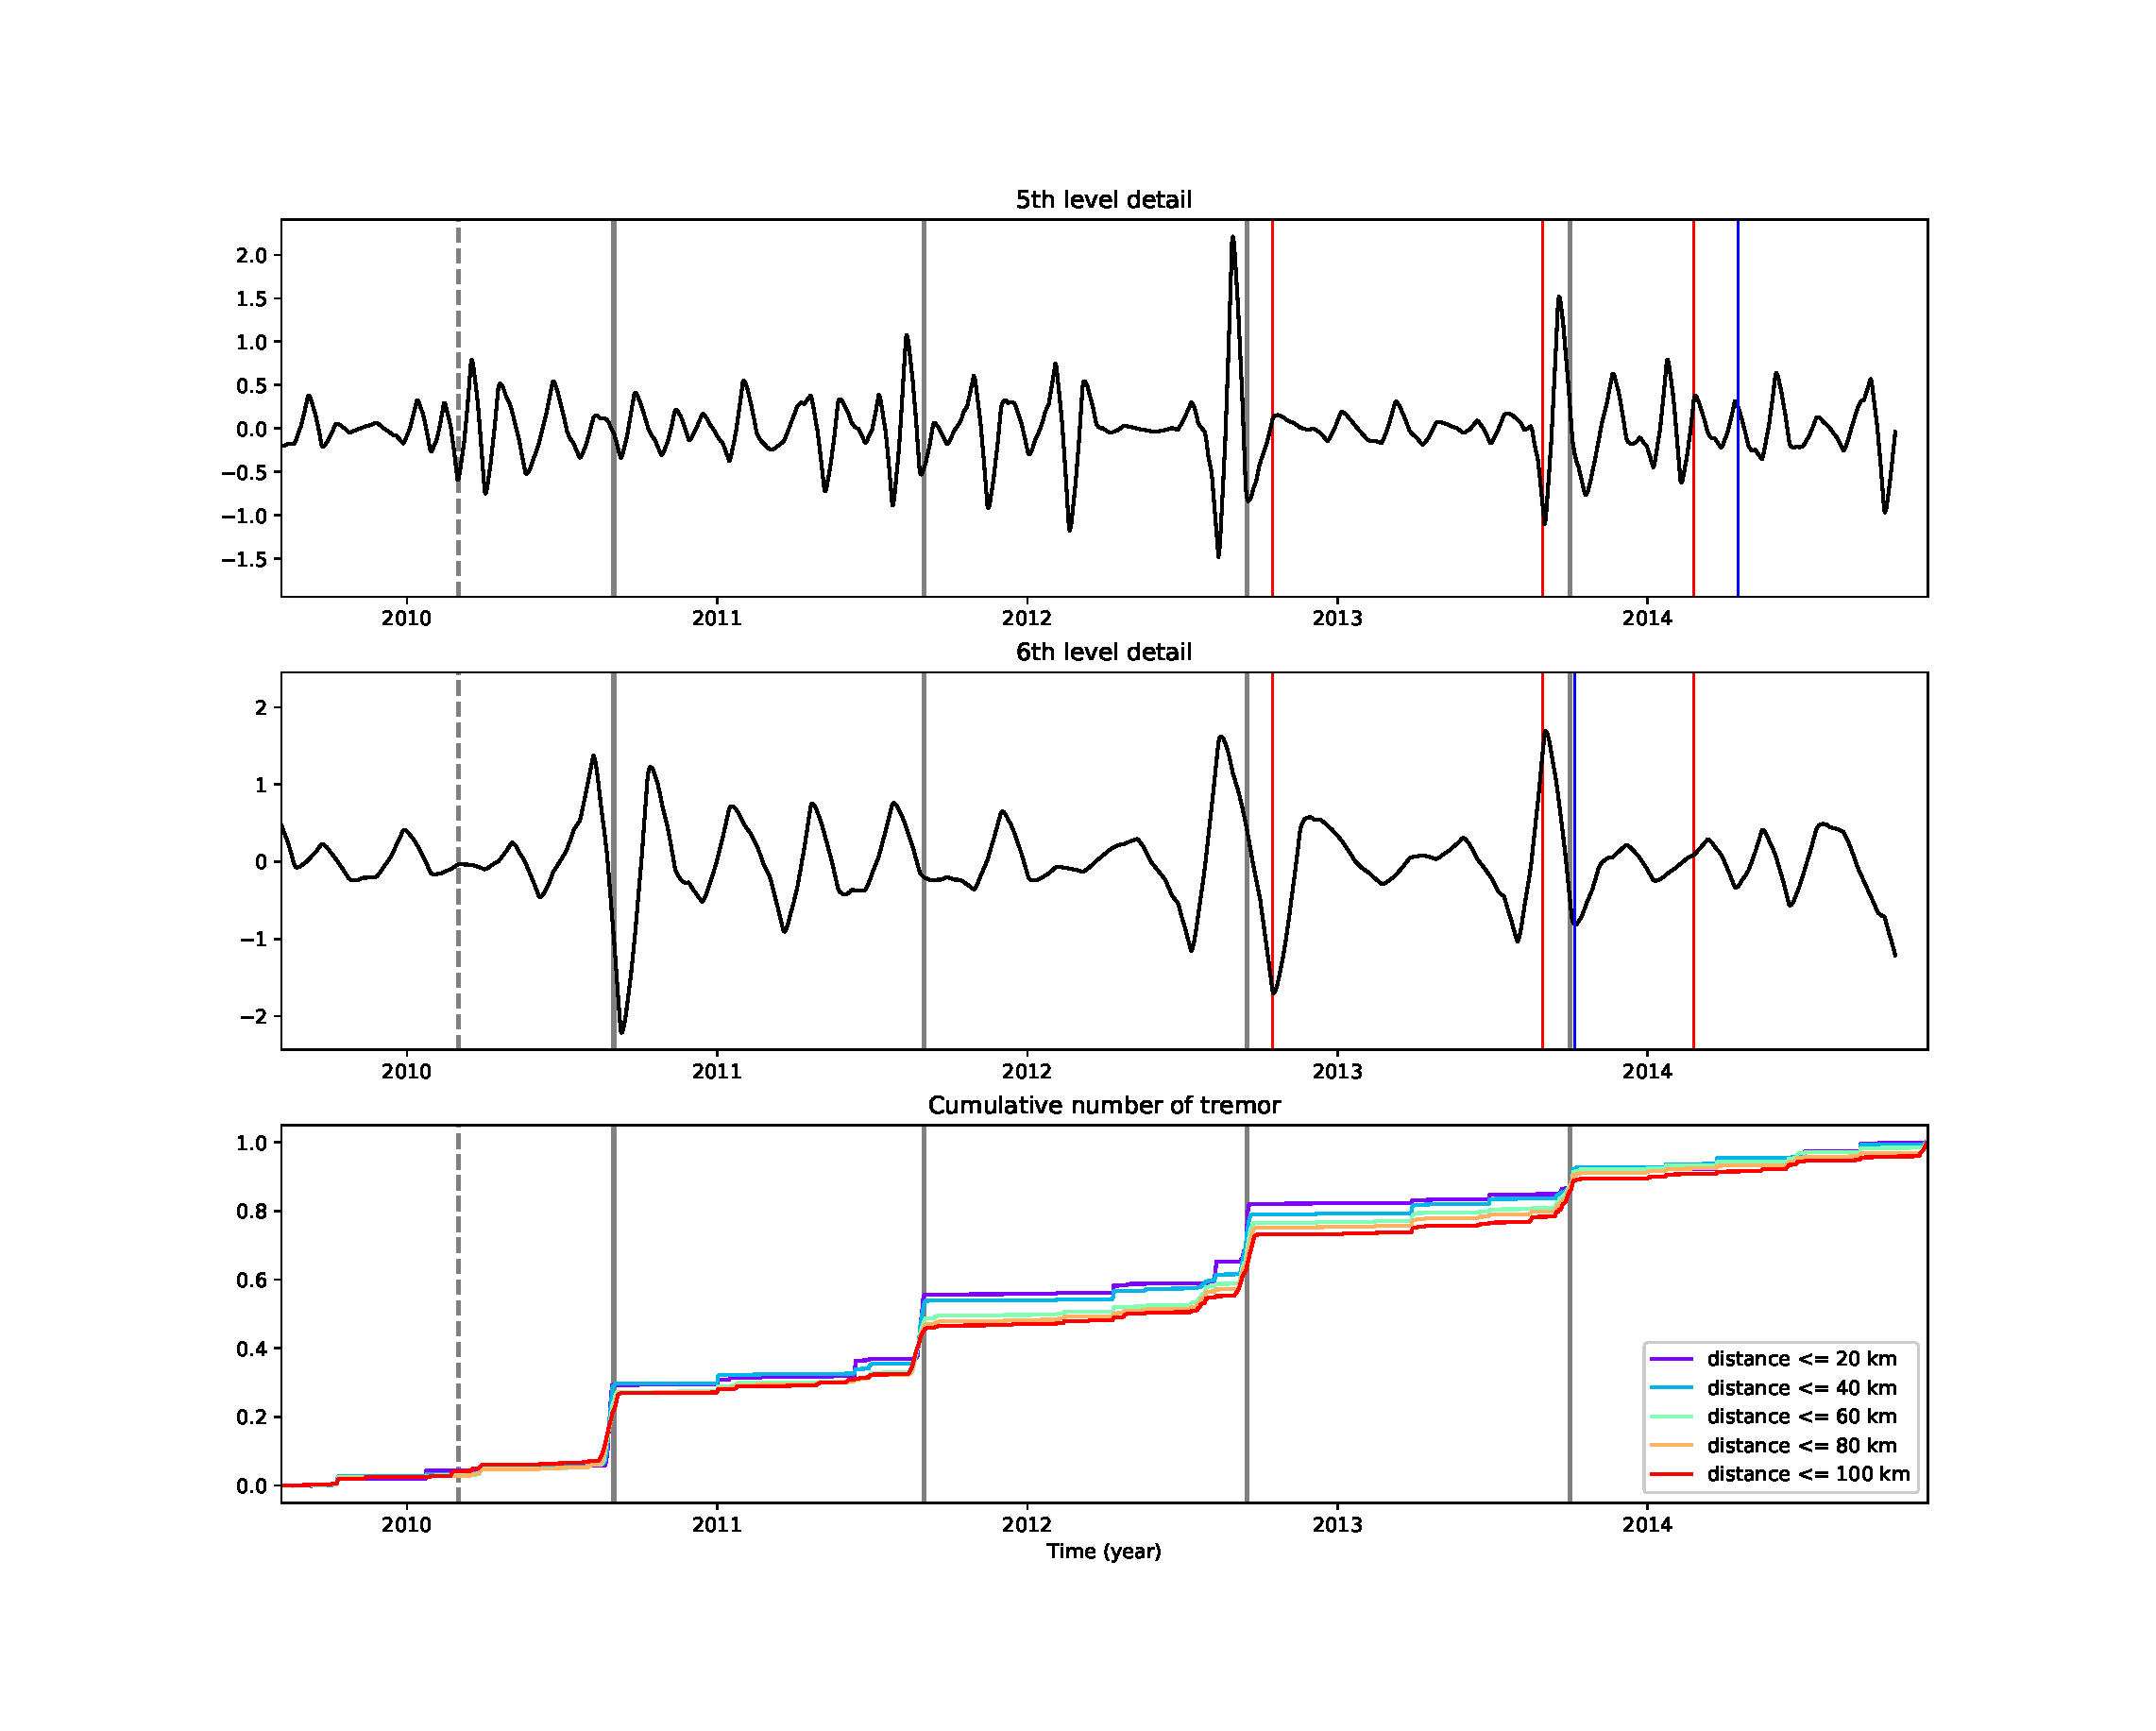
\includegraphics[width=300pt, trim={3.5cm 2.5cm 3.5cm 3cm}, clip]{Figures/slowslip_results/Figure_2.eps}
\captionsetup{type=figure}
\captionof{figure}{5\textsuperscript{th} and 6\textsuperscript{th} level details of the partial DWT analysis of the longitudinal component of station PGC5 (top and middle panel), and cumulative number of tremor
recorded around the GPS station (bottom panel). The red bars correspond to the days where data were missing. The grey bars correspond to the timing of ETS events.}
\end{center}

The details of the MRA with the partial DWT have a somewhat 'shark fin' look, which is not entirely pleasing. Moreover, the number of days between two ETS events may not correspond to a multiple of a power of 2. Therefore, it would be easier to interpret the wavelet coefficients at each level if their dimensions was the same as the dimension of the original time series. Finally, it would be easier to associate the details and smooths of the MRA with the cumulative number of tremor recorded if they were associated with zero phase filters. Therefore, in the following, we carried out a MODWT analysis on the same time series. \\

The wavelet coefficients for level 1 to 6 are shown in Figure 19.3. We can clearly see peaks corresponding to the January 2007, May 2009, August 2010, September 2012, and September 2013 ETS events in both the level 5 and level 6 coefficients. A peak corresponding to the May 2008 ETS event can be seen in the level 5 coefficients. However, it is still difficult to observe the August 2011 ETS event in the wavelet coefficients. \\

\begin{center}
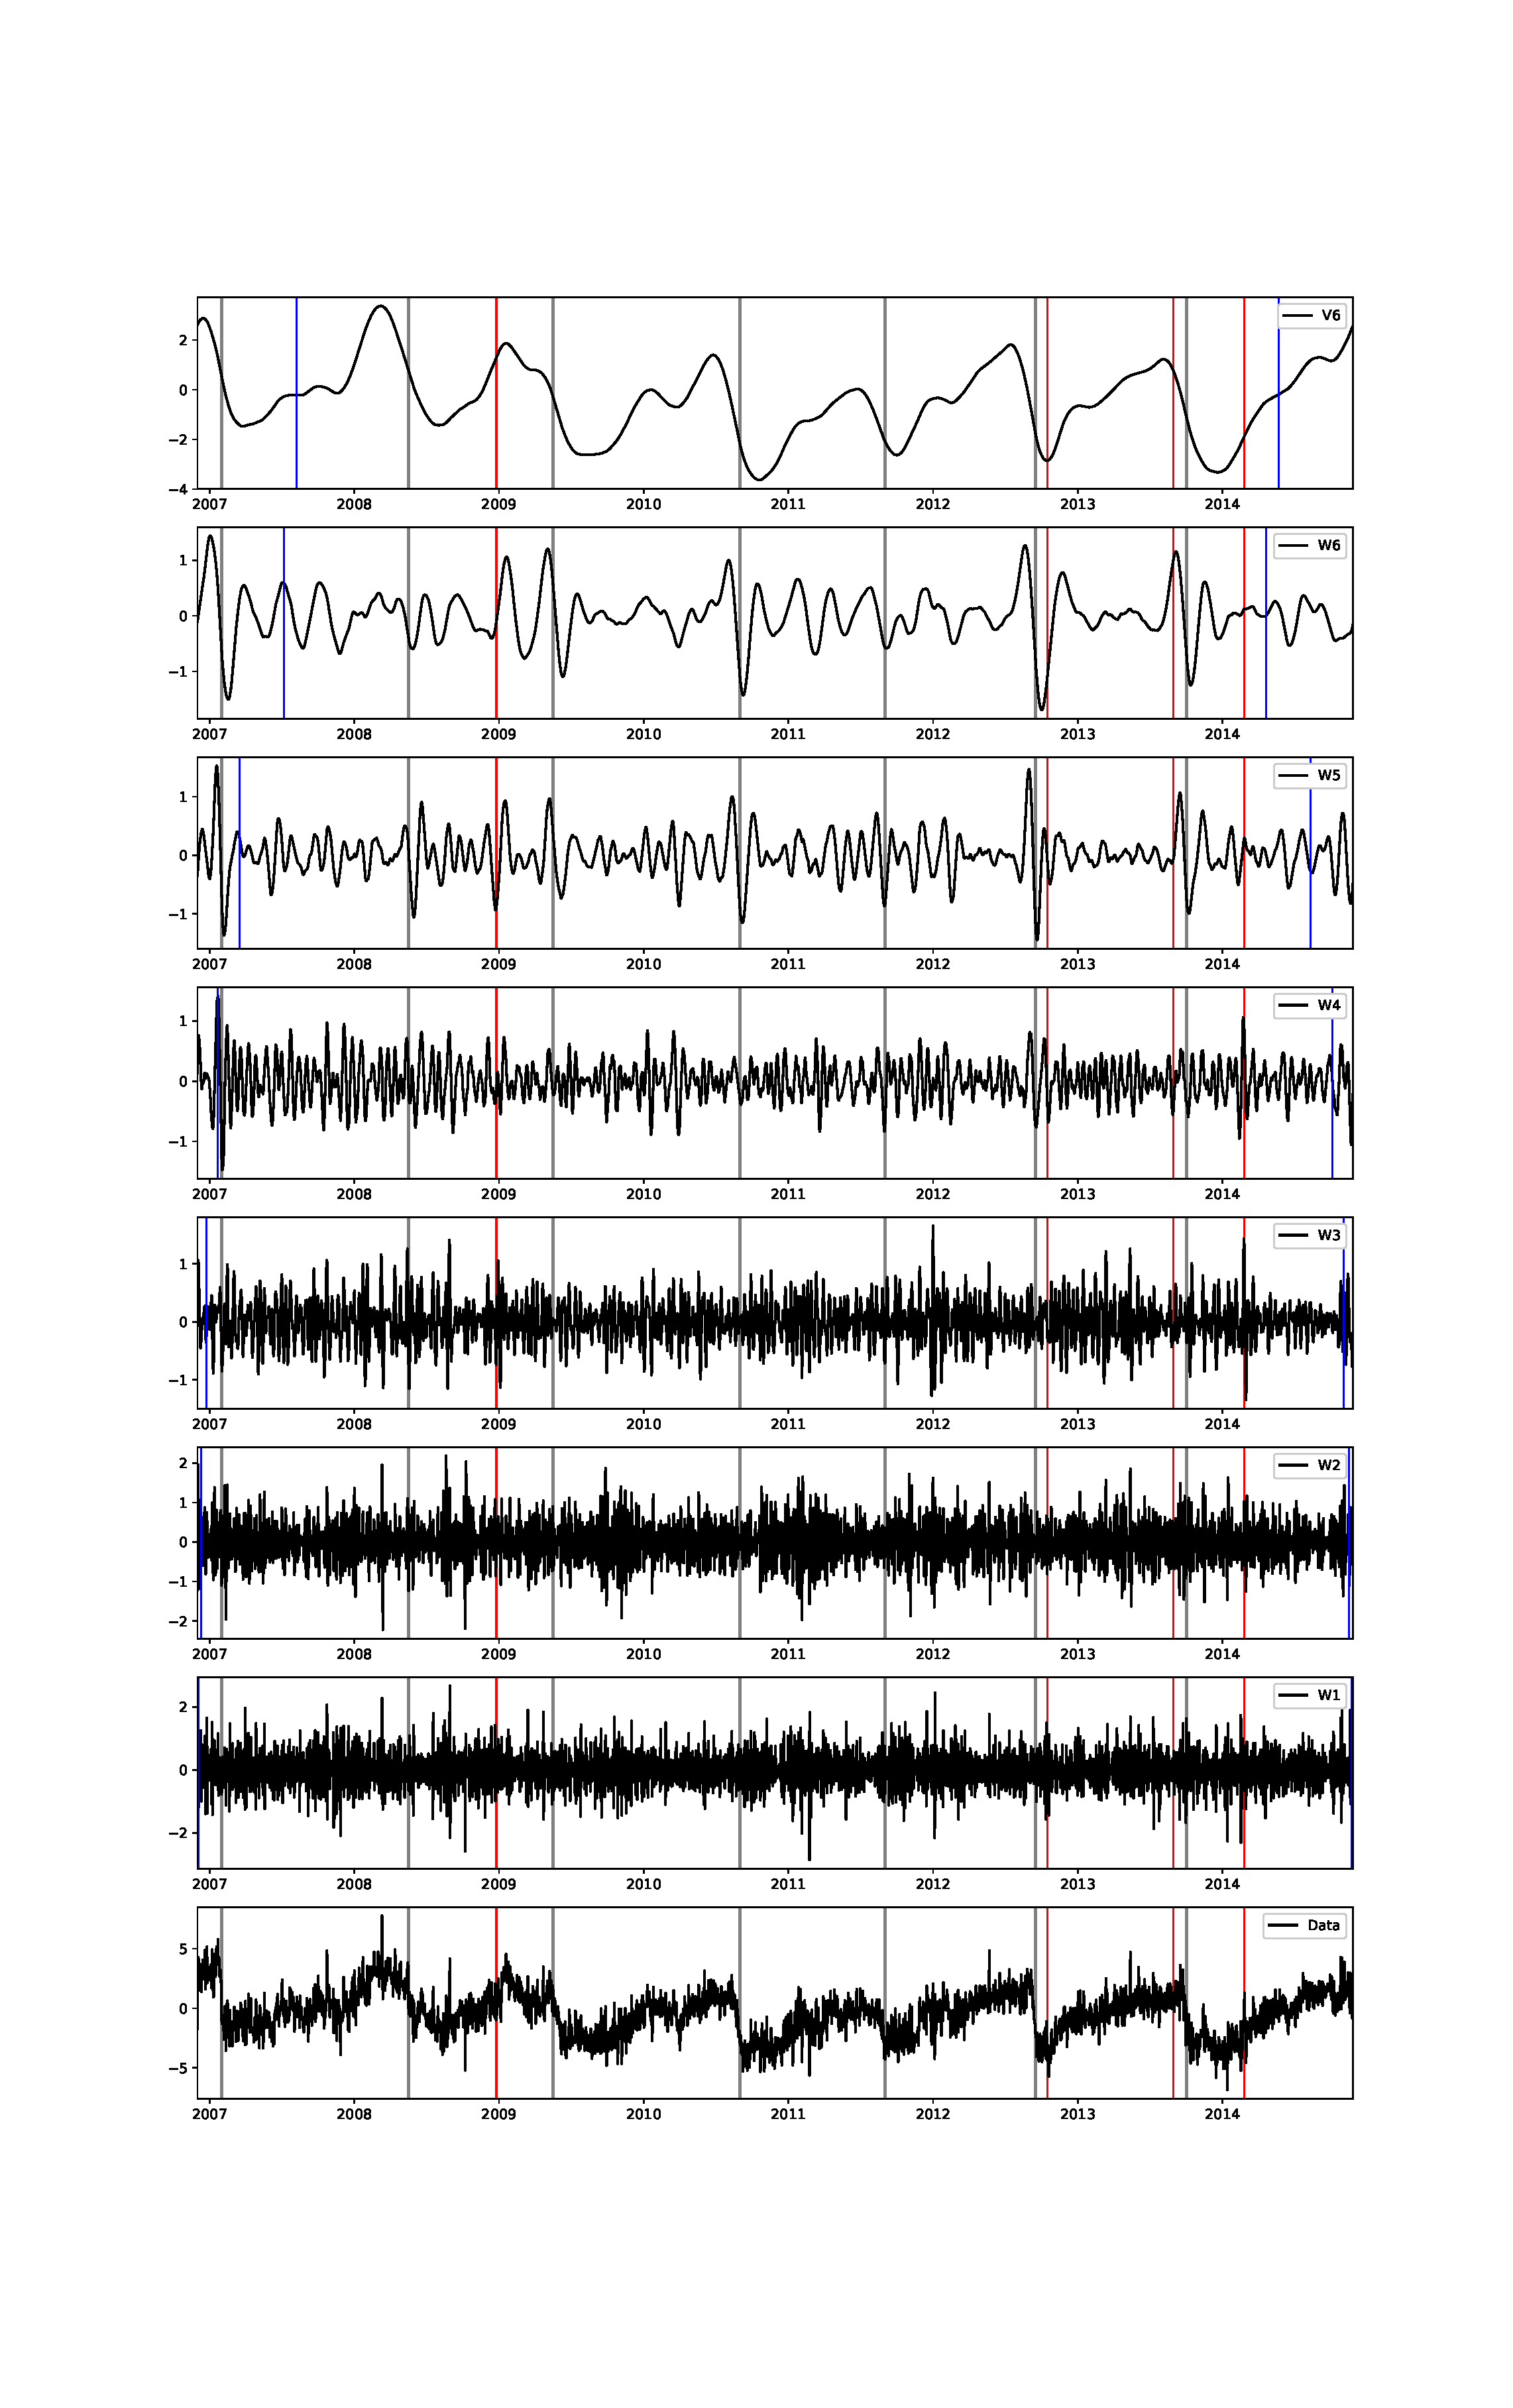
\includegraphics[width=300pt]{Figures/slowslip_results/Figure_3.eps}
\captionsetup{type=figure}
\captionof{figure}{Partial MODWT wavelet coefficients up to level 6.}
\end{center}

Finally, the 5\textsuperscript{th} and 6\textsuperscript{th} level details of the MRA are plotted with the cumulative number of tremor in Figure 19.4. Peaks corresponding to the August 2010, September 2012 and September 2013 ETS events can clearly be seen in both the 5\textsuperscript{th} and the 6\textsuperscript{th} level details. Peaks that could corresponds to the August 2011 ETS event, and a small inter-ETS event in March 2010, can also be seen in the 5\textsuperscript{th} level detail, but this is less obvious than for the other ETS events.

\begin{center}
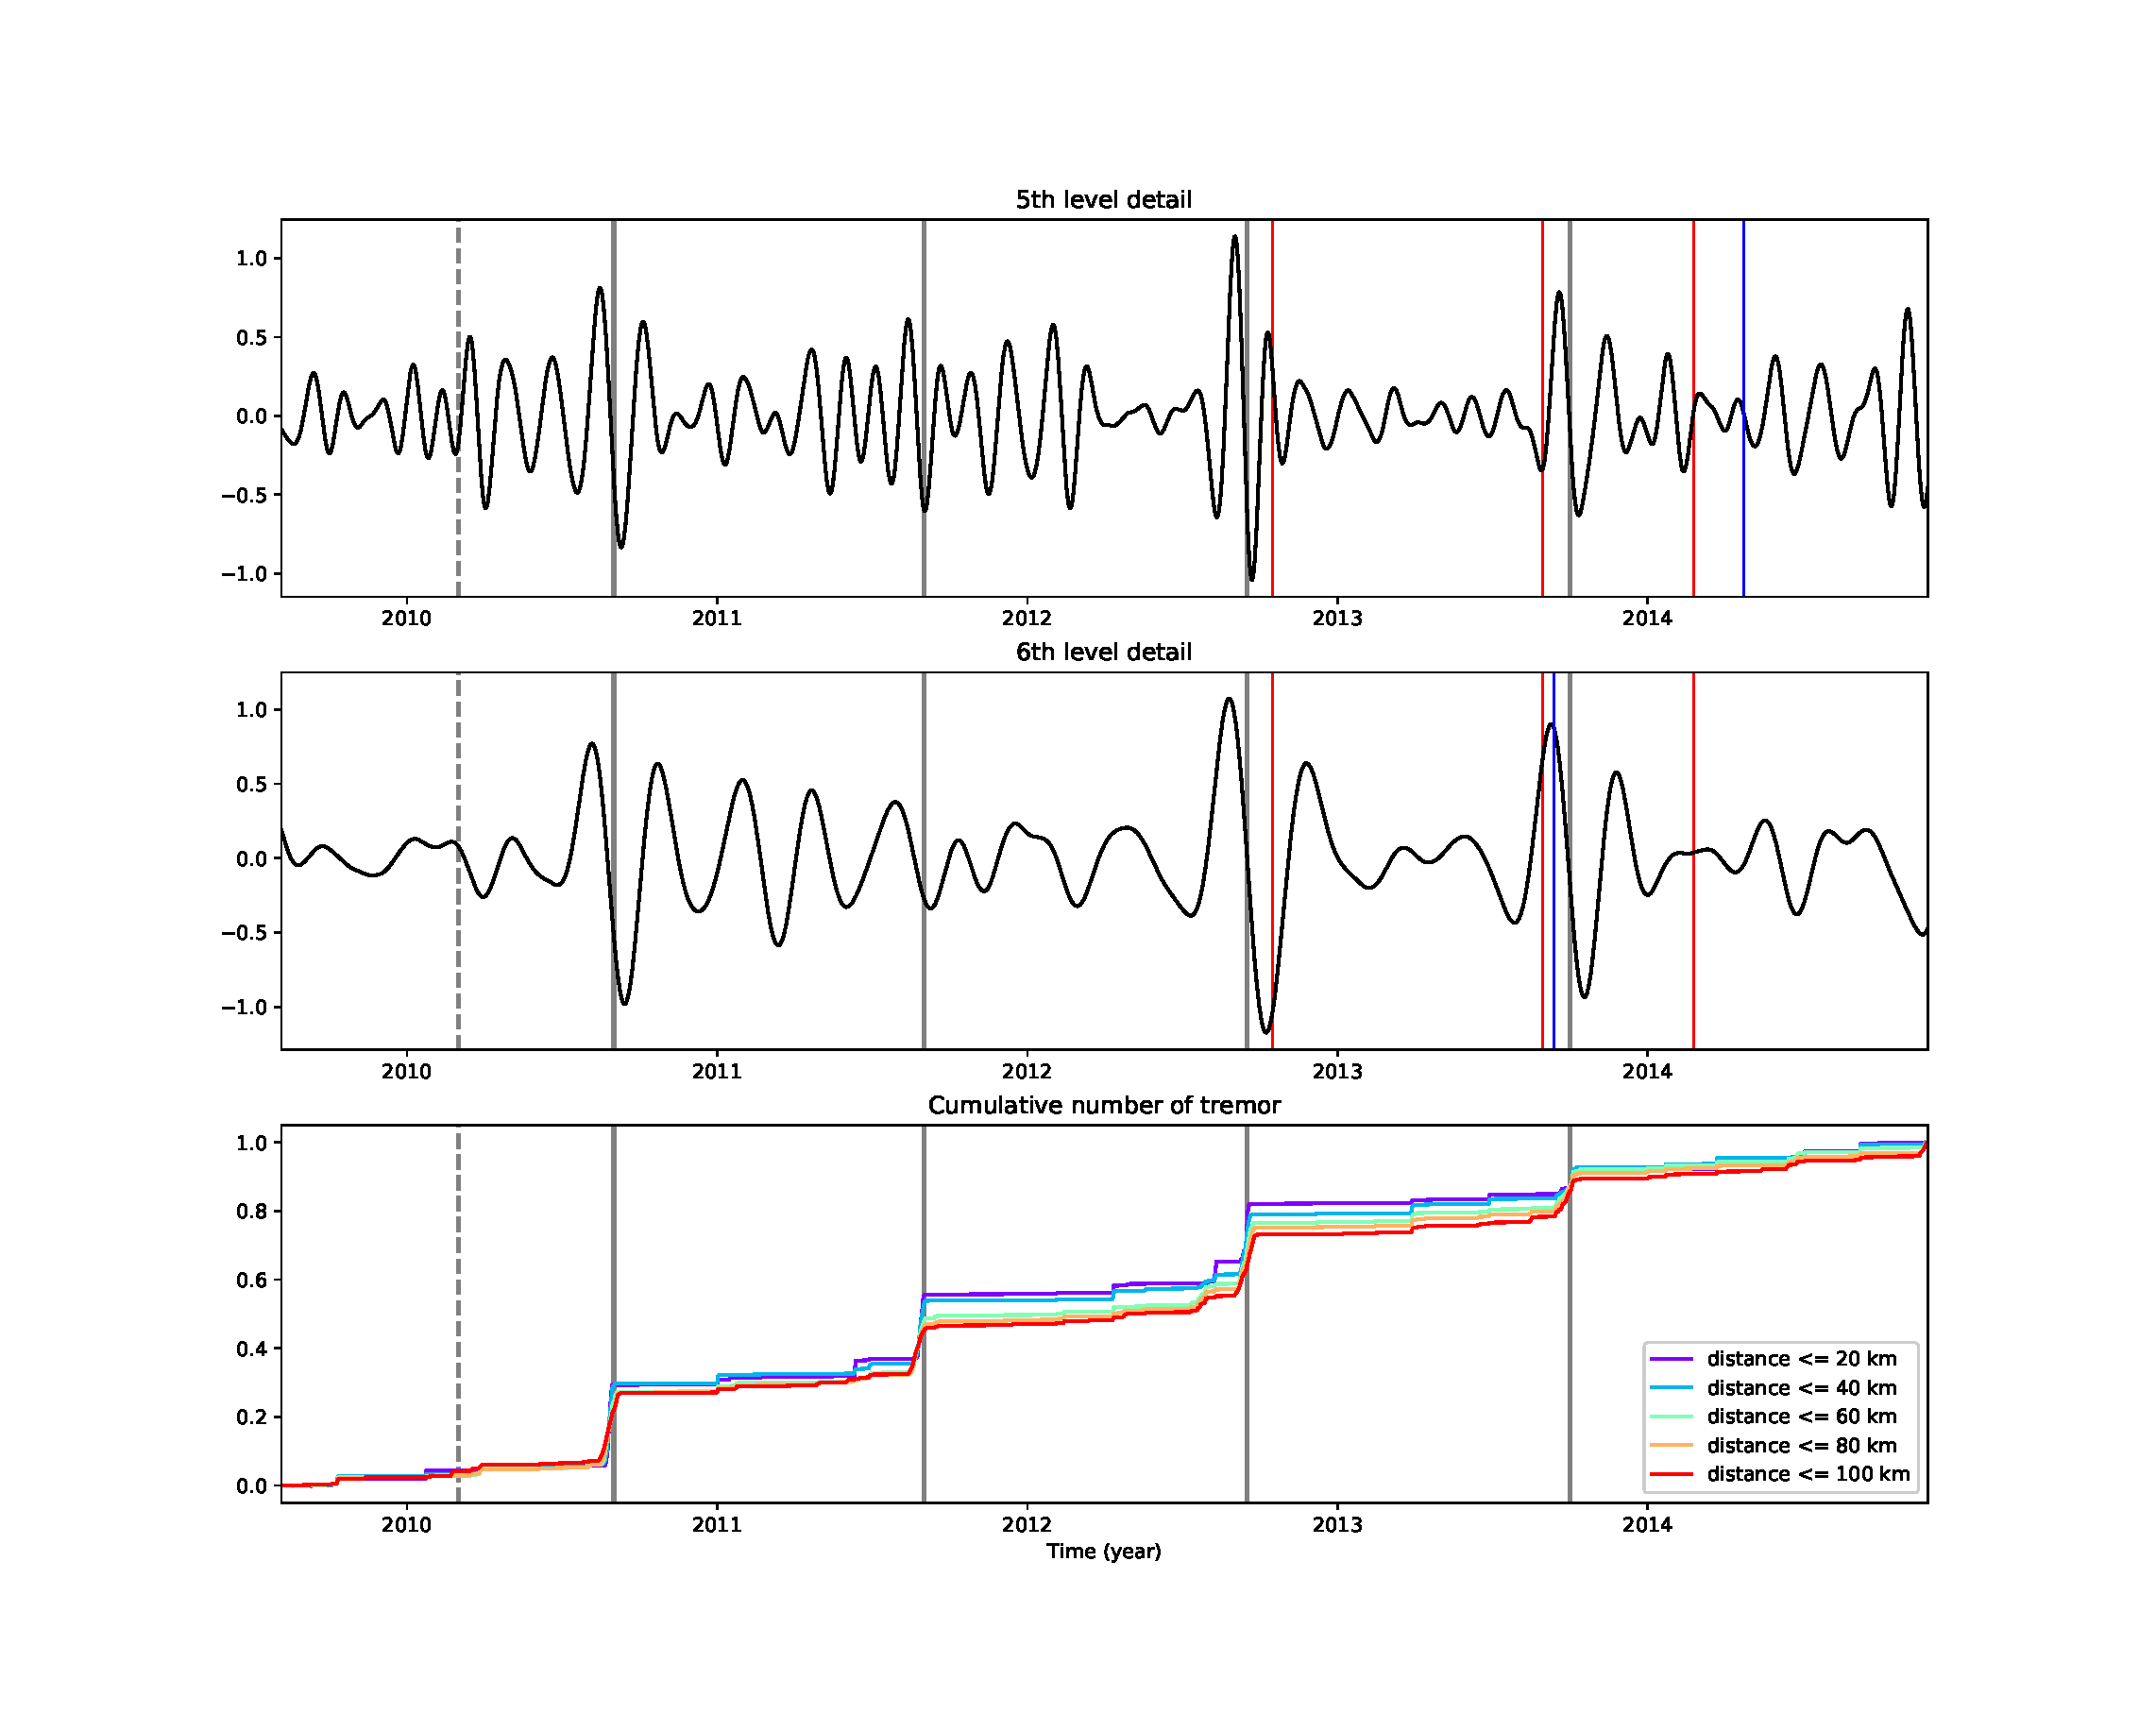
\includegraphics[width=300pt]{Figures/slowslip_results/Figure_4.eps}
\captionsetup{type=figure}
\captionof{figure}{5\textsuperscript{th} and 6\textsuperscript{th} level details of the partial MODWT analysis (top and middle panel), and cumulative number of tremor
recorded around the GPS station (bottom panel).}
\end{center}

We did a similar analysis with the GPS stations CLRS, CUSH, FRID, PNCL, PTAA, and SQIM, all located in the Olympic Peninsula, or on Vancouver Island, and we found similar results.

\chapter{Discussion and things to do}

Change point detection: Can we detect a big ETS event starting, and when can we detect it? Before it becomes obvious due to the tremor recordings? We could test other wavelets (Daubechies with extremal phase may be a good idea), or look at the wavelet variance (see paper by Eric Moulines - Kouamo et al., 2011, with correction of the mistake in Percival's paper).

Plot of the cumulative number of tremor: How to get the exact timing of the inflection point / change point for putting it on the wavelet plot?

\end{document}
